\section{Remote Attestation}
\label{sec:attestation}

A remote party can undergo an \textit{attestation} process to convince itself
that it is communicating with a specific enclave running in a secure
environment.

\begin{figure}[hbt]
  \center{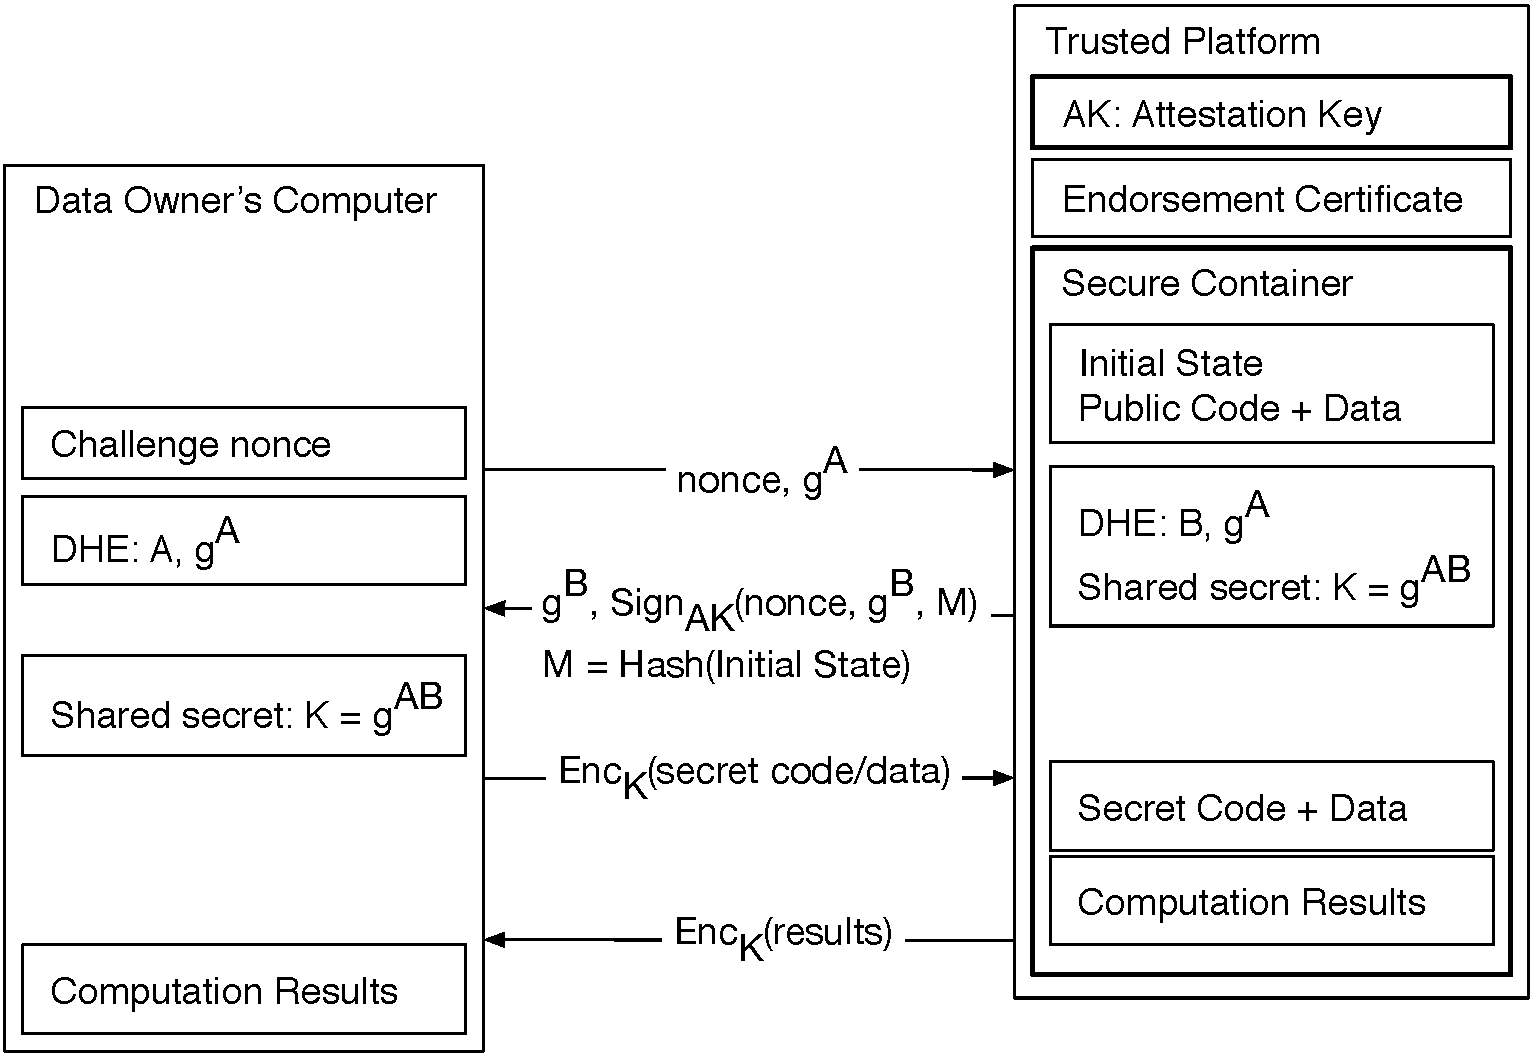
\includegraphics[width=85mm]{figures/generic_attestation.pdf}}
  \caption{
    Software attestation proves to a remote computer that it is communicating
    with a specific secure container hosted by a trusted platform. The proof is
    an attestation signature produced by the platform's secret attestation key.
    The signature covers the container's initial state, a challenge nonce
    produced by the remote computer, and a message produced by the container.
  }
  \label{fig:generic_attestation}
\end{figure}


The remote party starts the process by generating a random
challenge and sending it to the enclave.

The enclave asks the CPU to produce an \textit{enclave report}, which contains
the attestation challenge, the enclave's measurement value, an
enclave-generated 256-byte message, and an HMAC
 with a symmetric key shared between the CPU and a special
\textit{signing enclave} produced by Intel. The untrusted system software
executes the signing enclave, which verifies the report and produces an
\textit{attestation signature} that covers the challenge and the enclave's
measurement.

The remote party receives the attestation signature and the CPU's attestation
certificate, and

\subsection{Enclave Measurement}
\label{sec:measurement}

% SGX Enclave Control Structure (SECS): SGX S 2.6.1

The enclave measurement process uses the MRENCLAVE field in the SECS of the
enclave being measured. MRENCLAVE holds a 32-byte SHA-256 signature.

% ECREATE: SGX S 2.6.3, SGX S 5.3 ECREATE

The ECREATE instruction initializes the MRENCLAVE field in the newly created
SECS using the SHA-256 initialization algorithm, then extends the hash with
the ``ECREATE'' string, followed by the SSAFRAMESIZE and SIZE fields in the
SECS.

\begin{table}[hbt]
  \center{\begin{tabularx}{\columnwidth}{| r | r | X |}
  \hline
  \textbf{Offset} & \textbf{Size} & \textbf{Description}\\
  \hline
  0 & 8 & "ECREATE\textbackslash{}0" \\
  \hline
  8 & 8 & SECS.SSAFRAMESIZE \\
  \hline
  16 & 8 & SECS.SIZE \\
  \hline
  32 & 8 & 32 zero (0) bytes \\
  \hline
  \end{tabularx}}
  \caption{
    Data extended into MRENCLAVE by the ECREATE instruction.
  }
  \label{fig:ecreate_mrenclave}
\end{table}

% EADD and EEXTEND Interaction: SGX S 3.1.1
% EADD: SGX S 5.3 EADD

The EADD instruction extends the MRENCLAVE field in the enclave's SECS with the
``EADD'' string, followed by the page's linear address (relative to the start
of the enclave), and the first 48 bytes of the SECINFO structure that contains
the R, W, X values for the page's EPCM entry.

\begin{table}[hbt]
  \center{\begin{tabularx}{\columnwidth}{| r | r | X |}
  \hline
  \textbf{Offset} & \textbf{Size} & \textbf{Description}\\
  \hline
  0 & 8 &
  "EADD\textbackslash{}0\textbackslash{}0\textbackslash{}0\textbackslash{}0" \\
  \hline
  8 & 8 & PAGEINFO.LINADDR \\
  \hline
  16 & 48 & SECINFO (first 48 bytes) \\
  \hline
  \end{tabularx}}
  \caption{
    Data extended into MRENCLAVE by the EADD instruction.
  }
  \label{fig:eadd_mrenclave}
\end{table}

% EEXTEND: SGX S 5.3 EEXTEND

The EEXTEND instruction extends the MRENCLAVE field in the enclave's SECS with
the ``EEXTEND'' string, followed by the linear address of the 256-byte chunk
(relative to the start of the enclave).

\begin{table}[hbt]
  \center{\begin{tabularx}{\columnwidth}{| r | r | X |}
  \hline
  \textbf{Offset} & \textbf{Size} & \textbf{Description}\\
  \hline
  0 & 8 & "EEXTEND\textbackslash{}0" \\
  \hline
  8 & 8 & ENCLAVEOFFSET \\
  \hline
  16 & 48 & 48 zero (0) bytes \\
  \hline
  \hline
  64 & 64 & bytes 0 - 64 in the chunk \\
  \hline
  \hline
  128 & 64 & bytes 64 - 128 in the chunk \\
  \hline
  \hline
  192 & 64 & bytes 128 - 192 in the chunk \\
  \hline
  \hline
  256 & 64 & bytes 192 - 256 in the chunk \\
  \hline
  \end{tabularx}}
  \caption{
    Data extended into MRENCLAVE by the EEXTEND instruction.
  }
  \label{fig:eextend_mrenclave}
\end{table}

% EINIT: SGX S 5.3 EINIT

The EINIT instruction

\subsection{The Attestation Process}


% EINIT Token Structure (EINITTOKEN): SGX S 2.6.8



% Enclave Signature Structure (SIGSTRUCT): SGX S 2.6.7


% Internal CREGs: SGX S 5.1.4

